\chapter{Metodologia}
\label{chap:metodologia}


\section{Series Temporais}
Series Temporais são observações sequenciais de um conjunto de amostras, essas observações são feitas ao longo
do tempo. As técnicas aplicadas, que serão apresentadas a seguir, são uteis para predizer valores futuros da serie
\cite{Mesquita_2019}. A Figura \ref{fig:serie} mostra um exemplo de serie temporal.

\begin{figure}[h]
    \centering
    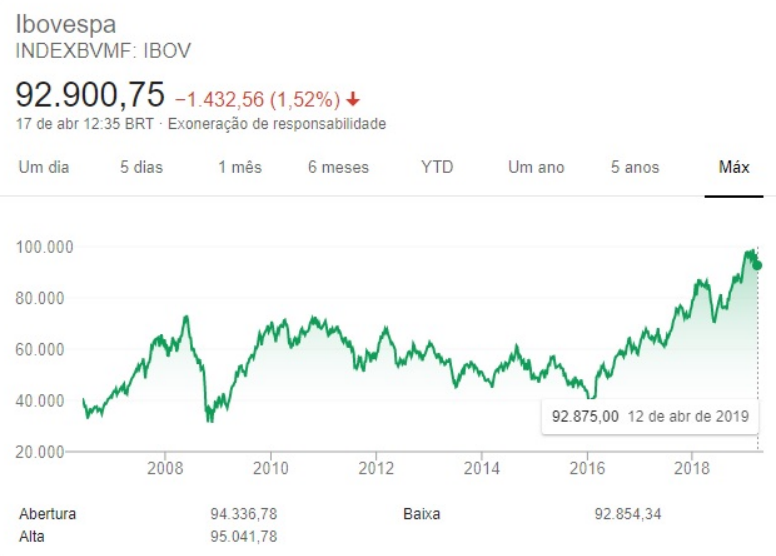
\includegraphics[width=10cm]{figuras/SVM_1.png}
    \caption{Ativos da bola de valore. Figura de \cite{Mesquita_2019}.}
    \label{fig:serie}
\end{figure}



\subsection{AR}

\subsection{ARMA}

\subsection{ARIMA}
